\documentclass[a4paper]{article}\usepackage[]{graphicx}\usepackage[]{color}
% maxwidth is the original width if it is less than linewidth
% otherwise use linewidth (to make sure the graphics do not exceed the margin)
\makeatletter
\def\maxwidth{ %
  \ifdim\Gin@nat@width>\linewidth
    \linewidth
  \else
    \Gin@nat@width
  \fi
}
\makeatother

\definecolor{fgcolor}{rgb}{0.345, 0.345, 0.345}
\makeatletter
\@ifundefined{AddToHook}{}{\AddToHook{package/xcolor/after}{\definecolor{fgcolor}{rgb}{0.345, 0.345, 0.345}}}
\makeatother
\newcommand{\hlnum}[1]{\textcolor[rgb]{0.686,0.059,0.569}{#1}}%
\newcommand{\hlstr}[1]{\textcolor[rgb]{0.192,0.494,0.8}{#1}}%
\newcommand{\hlcom}[1]{\textcolor[rgb]{0.678,0.584,0.686}{\textit{#1}}}%
\newcommand{\hlopt}[1]{\textcolor[rgb]{0,0,0}{#1}}%
\newcommand{\hlstd}[1]{\textcolor[rgb]{0.345,0.345,0.345}{#1}}%
\newcommand{\hlkwa}[1]{\textcolor[rgb]{0.161,0.373,0.58}{\textbf{#1}}}%
\newcommand{\hlkwb}[1]{\textcolor[rgb]{0.69,0.353,0.396}{#1}}%
\newcommand{\hlkwc}[1]{\textcolor[rgb]{0.333,0.667,0.333}{#1}}%
\newcommand{\hlkwd}[1]{\textcolor[rgb]{0.737,0.353,0.396}{\textbf{#1}}}%
\let\hlipl\hlkwb

\usepackage{framed}
\makeatletter
\newenvironment{kframe}{%
 \def\at@end@of@kframe{}%
 \ifinner\ifhmode%
  \def\at@end@of@kframe{\end{minipage}}%
  \begin{minipage}{\columnwidth}%
 \fi\fi%
 \def\FrameCommand##1{\hskip\@totalleftmargin \hskip-\fboxsep
 \colorbox{shadecolor}{##1}\hskip-\fboxsep
     % There is no \\@totalrightmargin, so:
     \hskip-\linewidth \hskip-\@totalleftmargin \hskip\columnwidth}%
 \MakeFramed {\advance\hsize-\width
   \@totalleftmargin\z@ \linewidth\hsize
   \@setminipage}}%
 {\par\unskip\endMakeFramed%
 \at@end@of@kframe}
\makeatother

\definecolor{shadecolor}{rgb}{.97, .97, .97}
\definecolor{messagecolor}{rgb}{0, 0, 0}
\definecolor{warningcolor}{rgb}{1, 0, 1}
\definecolor{errorcolor}{rgb}{1, 0, 0}
\makeatletter
\@ifundefined{AddToHook}{}{\AddToHook{package/xcolor/after}{
\definecolor{shadecolor}{rgb}{.97, .97, .97}
\definecolor{messagecolor}{rgb}{0, 0, 0}
\definecolor{warningcolor}{rgb}{1, 0, 1}
\definecolor{errorcolor}{rgb}{1, 0, 0}
}}
\makeatother
\newenvironment{knitrout}{}{} % an empty environment to be redefined in TeX

\usepackage{alltt}
\usepackage{fullpage}
\usepackage{float}
\usepackage{booktabs}
\usepackage{tikz-cd}
\usepackage{amsmath}
\usepackage[T1]{fontenc}
\usepackage{hyperref}
\hypersetup{
    colorlinks = true,
    linkcolor = blue,
    citecolor = blue,
    urlcolor  = blue
    }

\urlstyle{same}
\usepackage{graphicx}
\graphicspath{{./figures//}}

\usepackage{listings}
\lstset{
basicstyle=\small\ttfamily,
columns=flexible,
breaklines=true
}
\usepackage{fancyvrb,newverbs,xcolor}
\definecolor{cverbbg}{gray}{0.93}

\setlength\parindent{24pt}

\usepackage[bibstyle=authoryear,
citestyle=authoryear-ibid, backend=bibtex]{biblatex}
\addbibresource{mybib.bib}

\title{The Costs of Patronage:\\ Evidence from the British Empire\thanks{Original paper by Guo, Xu, published in American Economic Review 2018, 108(11), p. 3170 - 3198} \\ \vskip 0.4cm \normalsize Replication Analyis by Andreas Chmielowski for Econometrics III}

\date{\vspace{-5ex}}
\setlength{\parindent}{0em}
\IfFileExists{upquote.sty}{\usepackage{upquote}}{}
\begin{document}
%\SweaveOpts{concordance=TRUE}


\maketitle

\section{Introduction}
\hspace*{5mm} In the underlying paper, the author investigates how personal connections between bureaucrats and their superiors impact job appointment and performance under patronage, i.e. in a system where job appointment is completely at the discretion of the superior. The particular focus is on the appointment of colonial governors in the British Empire by the secretary of state. Did governors who had some \textit{predetermined} connection to the secretary of state (because they were relatives, they went to the same university, or they where both members of the aristocracy) treated preferentially (i.e. appointed to higher-paying colonies)? And did connected governors perform better (e.g. due to loyalty to their superior) or worse (e.g. due to lack of incentive)? The answers to these questions can inform how to organize appointment to public office best -- also nowadays -- and assess whether patronage in particular is an efficient way of doing it \parencite{guoxu2018}.

\hspace*{5mm} For the analysis, the author uses a dataset extracted from digitized historical personnel and public finance reports of the British Colonial Office from 1854 until 1966. These data capture both the variation in connectedness between a governor and a Secretary of State within a governor's term (ministerial changes in London) and variation in the extent of discretion of the Secretary due to a reform of the appointment mechanism of colonial governors in 1930 (the \textit{Warren-Fisher Reform}, which basically removed patronage). Data on connectedness between governors and Secretaries stems from genealogical and biographical sources and data on Governors' job performance comes from records of public revenues and expenditures of the colonies. The check for the robustness of the results, alternative performance measures are used: Social unrest in the colony, mentions and sentiments regarding particular governors in parliamentary debates, and the likelihood to receive a public award \parencite[p.3171 ff.]{guoxu2018}. 

\hspace*{5mm} The author's complete data and Stata code is readily available online and was used for this replication. Most variables are used from the dataset as they come, but others I had to derive first (e.g. certain grouped indices, means per quinnenial etc.) That is, there was not much data cleaning necessary because the published data were already in a pretty good shape. I recoded the whole analysis in \texttt{R}, because this is my primary language, and commented on all steps in the \texttt{R} script (attached in the submission). I also added some additional steps where I found them meaningful. In what follows I present my replication of the tables and comment on changes, where they occur. 

\section{Descriptive Statistics}

\hspace*{5mm} Tables~\ref{tab:descriptives1}~and~\ref{tab:descriptives2} reproduce panels A and B from Table 1 of \cite{guoxu2018} and show descriptive statistics on governors and officers. The pooled means for governors were obtained by first calculating the mean for each governor over the years of their mandate and then getting the mean over all governor means. For the particular years, only a single mean is necessary. The calculated statisticis are indeed the same as in the paper, except for some rounding errors. Interestingly, the dataset comes with 4,687 observations, but every time when the author refers to a statistic from the "full" dataset, he only uses 3,510 observations (filtered with a dummy variable called "full" in the data set). He does not explain what this is about, but I assume it has something to do with whether comprehensive information of a governors connectedness to the then-incumbent Secretary of State was available. All statistics in Tables~\ref{tab:descriptives1}~and~\ref{tab:descriptives2} only use these 3,510 observations. To each table, I add another column with the means of the pooled data with all 4,687 observations and find no large differences to the "full" sample.   
\begin{table}[!h]

\caption{\label{tab:descriptives1}Descriptive characteristics of governors}
\centering
\fontsize{7}{9}\selectfont
\begin{tabular}[t]{llllllll}
\toprule
\multicolumn{1}{c}{ } & \multicolumn{2}{c}{Pooled years} & \multicolumn{4}{c}{By year} & \multicolumn{1}{c}{unfiltered} \\
\cmidrule(l{3pt}r{3pt}){2-3} \cmidrule(l{3pt}r{3pt}){4-7} \cmidrule(l{3pt}r{3pt}){8-8}
  & Mean & SD & 1860 & 1900 & 1930 & 1960 & All\\
\midrule
Peerage & 0.086 & 0.280 & 0.048 & 0.154 & 0.027 & 0.000 & 0.071\\
Civil servant & 0.846 & 0.361 & 0.810 & 0.923 & 0.838 & 1.000 & 0.797\\
Military & 0.441 & 0.497 & 0.417 & 0.412 & 0.324 & 0.200 & 0.437\\
Politician & 0.088 & 0.283 & 0.167 & 0.128 & 0.027 & 0.000 & 0.078\\
Eton & 0.109 & 0.312 & 0.125 & 0.067 & 0.069 & 0.111 & 0.103\\
Oxford & 0.179 & 0.384 & 0.136 & 0.147 & 0.303 & 0.100 & 0.213\\
Cambridge & 0.151 & 0.358 & 0.103 & 0.194 & 0.242 & 0.600 & 0.153\\
Age at entry & 48.653 & 8.990 & 41.600 & 46.077 & 50.800 & 48.900 & 48.838\\
Years served & 4.221 & 3.655 & 5.500 & 4.897 & 4.081 & 2.700 & 3.511\\
Colonies served & 1.478 & 0.781 & 1.667 & 1.564 & 1.324 & 1.300 & 1.375\\
Observations & 456 & - & 42 & 39 & 37 & 10 & 456\\
\bottomrule
\end{tabular}
\end{table}

\begin{table}[!h]

\caption{\label{tab:descriptives2}Descriptive characteristics of British colonies}
\centering
\fontsize{7}{9}\selectfont
\begin{tabular}[t]{llllllll}
\toprule
\multicolumn{1}{c}{ } & \multicolumn{2}{c}{Pooled years} & \multicolumn{4}{c}{By year} & \multicolumn{1}{c}{unfiltered} \\
\cmidrule(l{3pt}r{3pt}){2-3} \cmidrule(l{3pt}r{3pt}){4-7} \cmidrule(l{3pt}r{3pt}){8-8}
  & Mean & SD & 1860 & 1900 & 1930 & 1960 & All\\
\midrule
(log) Total revenue & 12.309 & 2.185 & 10.85 & 12.639 & 13.135 & 15.961 & 12.232\\
Share customs revenue & 0.477 & 0.219 & 0.567 & 0.457 & 0.432 & 0.575 & 0.481\\
(log) Total expenditure & 12.333 & 2.166 & 10.88 & 12.552 & 13.237 & 15.965 & 12.236\\
(log) Population & 11.69 & 1.996 & 10.823 & 12.037 & 12.071 & 13.052 & 11.712\\
(log) Governorship salary & 7.929 & 0.796 & 7.74 & 7.962 & 8.079 & 8.878 & 7.958\\
Area tropics & 0.653 & 0.423 & 0.565 & 0.591 & 0.721 & 0.742 & 0.651\\
(log) Distance from London & 8.386 & 0.552 & 8.337 & 8.453 & 8.329 & 8.243 & 8.387\\
Observations & 3510 & - & - & - & - & - & 4687\\
Colonies & 70 & 42 & 39 & 37 & 10 & 71 & 70\\
\bottomrule
\end{tabular}
\end{table}


\hspace*{5mm} In Figures~\ref{fig:plot1}~and~\ref{fig:plot2}, I reproduce Figures 2 and 3 from the paper. Here, the author uses all observations (not only the "full" subset), which are replicated in the upper plots (blue). The red plots utilize only the full set (i.e. the "full" dummy equals 1). No qualitative differences can be observed. Especially Figure~\ref{fig:plot2} shows that, for a most of the time, salaries are indeed higher for connected governors. However, at this point nothing can be said about causality yet.    
\begin{figure}

{\centering 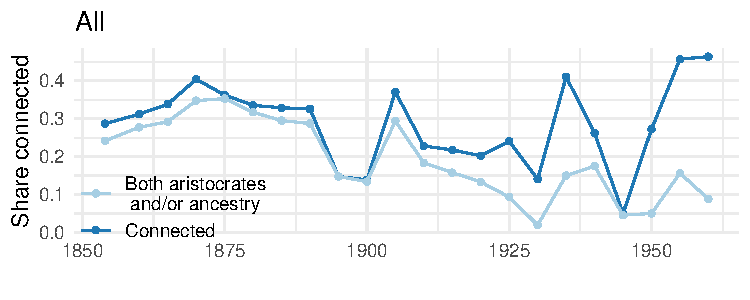
\includegraphics[width=\maxwidth]{figure/plot1-1} 
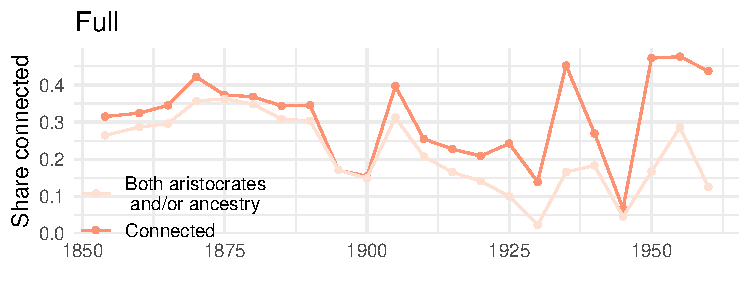
\includegraphics[width=\maxwidth]{figure/plot1-2} 

}

\caption[Share of governors connected to the secretary of state]{Share of governors connected to the secretary of state}\label{fig:plot1}
\end{figure}



\begin{figure}

{\centering 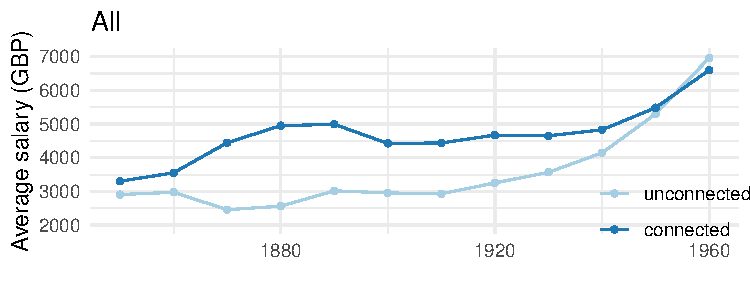
\includegraphics[width=\maxwidth]{figure/plot2-1} 
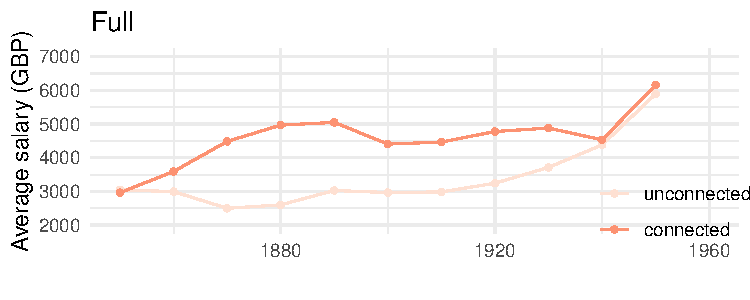
\includegraphics[width=\maxwidth]{figure/plot2-2} 

}

\caption[Average salary connected versus unconnected over time]{Average salary connected versus unconnected over time}\label{fig:plot2}
\end{figure}



\section{Results}
\subsection{Salary premium of social connections}
\hspace*{5mm} Table~\ref{tab:sal} shows the effect of all measures of predetermined connectedness considered in the paper on the governor salary, mirroring Table 2 from the paper. As governor FE, year FE and spell length FE are included in the regressions, it seems plausible that the source of variation left which is captured by connection is the variation on the side of the secretary of state -- personnel changes in the government in London. Especially the governor FE absorb variation from the possibility that time-invariant higher-skilled governors might earn higher salaries and be better connected, and the identification is therefore driven by connection changes of governors during their career. As before with the descriptive statistics, I included now all observations in column (7) (some of which have been nonetheless excluded due to missingness of relevant variables). The positive salary premium remains significant and stable also in this version of the sample.


% Table created by stargazer v.5.2.3 by Marek Hlavac, Social Policy Institute. E-mail: marek.hlavac at gmail.com
% Date and time: Wed, Sep 27, 2023 - 2:58:26 PM
\begin{table}[!htbp] \centering 
  \caption{Regressions of governor salaries on the connectedness to the secretary of state} 
  \label{tab:sal} 
\scriptsize 
\begin{tabular}{@{\extracolsep{5pt}}lccccccc} 
\\[-1.8ex]\hline 
\hline \\[-1.8ex] 
\\[-1.8ex] & \multicolumn{7}{c}{log governor salary} \\ 
\\[-1.8ex] & (1) & (2) & (3) & (4) & (5) & (6) & (7)\\ 
\hline \\[-1.8ex] 
 No. colonies served & 0.221$^{***}$ & 0.222$^{***}$ & 0.223$^{***}$ & 0.222$^{***}$ & 0.224$^{***}$ & 0.223$^{***}$ & 0.218$^{***}$ \\ 
  & (0.035) & (0.035) & (0.035) & (0.035) & (0.035) & (0.035) & (0.032) \\ 
  & & & & & & & \\ 
 Shared ancestors & 0.103$^{**}$ &  &  &  & 0.093$^{**}$ &  &  \\ 
  & (0.047) &  &  &  & (0.046) &  &  \\ 
  & & & & & & & \\ 
 Both aristocrats &  & 0.215$^{*}$ &  &  & 0.176 &  &  \\ 
  &  & (0.124) &  &  & (0.121) &  &  \\ 
  & & & & & & & \\ 
 Both Eton &  &  & 0.133$^{*}$ &  & 0.118 &  &  \\ 
  &  &  & (0.077) &  & (0.081) &  &  \\ 
  & & & & & & & \\ 
 Both Oxbridge &  &  &  & 0.072 & 0.073 &  &  \\ 
  &  &  &  & (0.047) & (0.045) &  &  \\ 
  & & & & & & & \\ 
 Connected &  &  &  &  &  & 0.097$^{***}$ & 0.087$^{***}$ \\ 
  &  &  &  &  &  & (0.036) & (0.027) \\ 
  & & & & & & & \\ 
\hline \\[-1.8ex] 
Mean of dep. var & 7.929 & 7.929 & 7.929 & 7.929 & 7.929 & 7.929 & 7.958 \\ 
Year FE & Yes & Yes & Yes & Yes & Yes & Yes & Yes \\ 
Governor FE & Yes & Yes & Yes & Yes & Yes & Yes & Yes \\ 
Spell lengths FE & Yes & Yes & Yes & Yes & Yes & Yes & Yes \\ 
Observations & 3,510 & 3,510 & 3,510 & 3,510 & 3,510 & 3,510 & 4,290 \\ 
\hline 
\hline \\[-1.8ex] 
\textit{Note:}  & \multicolumn{7}{r}{$^{*}$p$<$0.1; $^{**}$p$<$0.05; $^{***}$p$<$0.01} \\ 
\end{tabular} 
\end{table} 


\subsection{Transfers and connectedness}
\hspace*{5mm} Columns (1) and (2) of Table~\ref{tab:tran}, which replicates the results from Table 3 in the paper, imply that transfers to higher paying colonies were the main driver of the previously observed salary premia of connectedness: The introduction of colony FE decreases the coefficient of connectedness and makes it insignificant, which might indicate that the difference in salary induced by connectedness is mediated via colony characteristics. Column (3) shows the effect of connectedness on the log initial revenue, which, according to the author, is an indicator of the colony size. However, in the provided Stata code, the calculation of this log initial revenue is conducted by first grouping observations by colony ID and them calculating the minimum log revenue for each colony. I do not find this calculation to be correct and therefore repeat this estimation in column (6) with the actual initial log revenue of every colony when a governor started his mandate there\footnote{If revenue is a measure of colony size and larger size means higher salary, I argue that if a secretary of state decided to treat a particular governor preferentially, he whould appoint him to a colony on basis of the revenue \textit{in that particular year} when the decision was made.}. The effect of connectedness is significant and virtually the same as in column (3). Columns (4) and (5) show the effect of connectedness on whether the area is in the tropics and on the log distance of the colony to London, respectively, and both are insignificant. Column (7) shows the same regression as (6), but again with all observations (not only the "full" sample).

% Table created by stargazer v.5.2.3 by Marek Hlavac, Social Policy Institute. E-mail: marek.hlavac at gmail.com
% Date and time: Wed, Sep 27, 2023 - 2:58:26 PM
\begin{table}[!htbp] \centering 
  \caption{Transfers and connectedness to the Secretary of State} 
  \label{tab:tran} 
\scriptsize 
\begin{tabular}{@{\extracolsep{5pt}}lccccccc} 
\\[-1.8ex]\hline 
\hline \\[-1.8ex] 
 & \multicolumn{2}{c}{log governor salary} & \multicolumn{3}{c}{Colony Fixed effects} & \multicolumn{2}{c}{actual initial rev} \\ 
\\[-1.8ex] & (1) & (2) & (3) & (4) & (5) & (6) & (7)\\ 
\hline \\[-1.8ex] 
 No. colonies served & 0.223$^{***}$ & 0.035$^{*}$ & 0.737$^{***}$ & $-$0.017 & 0.063$^{**}$ & 0.673$^{***}$ & 0.723$^{***}$ \\ 
  & (0.035) & (0.020) & (0.095) & (0.025) & (0.029) & (0.084) & (0.081) \\ 
  & & & & & & & \\ 
 Connected & 0.097$^{***}$ & 0.011 & 0.177$^{*}$ & 0.014 & $-$0.019 & 0.179$^{**}$ & 0.134$^{*}$ \\ 
  & (0.036) & (0.018) & (0.099) & (0.029) & (0.033) & (0.078) & (0.077) \\ 
  & & & & & & & \\ 
\hline \\[-1.8ex] 
Mean of dep. var & 7.929 & 7.929 & 10.743 & 0.653 & 8.386 & 12.107 & 11.981 \\ 
Year FE & Yes & Yes & Yes & Yes & Yes & Yes & Yes \\ 
Governor FE & Yes & Yes & Yes & Yes & Yes & Yes & Yes \\ 
Colony FE & - & Yes & - & - & - & - & - \\ 
Spell lengths FE & Yes & Yes & Yes & Yes & Yes & Yes & Yes \\ 
Observations & 3,510 & 3,510 & 3,510 & 3,510 & 3,510 & 3,510 & 3,550 \\ 
\hline 
\hline \\[-1.8ex] 
\textit{Note:}  & \multicolumn{7}{r}{$^{*}$p$<$0.1; $^{**}$p$<$0.05; $^{***}$p$<$0.01} \\ 
\end{tabular} 
\end{table} 

\hspace*{5mm} Given that transfers to high-salary colonies are the primary way for secretaries to treat connected governors preferentially, we see in columns (3) and (6) of Table~\ref{tab:tran} that connectedness is significantly associated with larger colonies. I decided to augment this argument by conducting a proper mediation analysis as shown in Figure~\ref{triangle}. That is, I assess whether channel \textit{c} is actually fully or only partly mediated by the colony size. I do not consider the other two colony characteristics, area on tropics and log distance to London, as their association with connectedness is insignificant. The results of the mediation analysis can be found in Tables~\ref{tab:mediation1} and \ref{tab:mediation2}. For the log initial revenue, I included my own calculated measure (because I think it is the right one) and I included the same FE and controls as in Table~\ref{tab:tran}. The mediation analysis shows that only 44\% of the the salary premium due to connectedness is mediated by colony size, which means that other colony characteristics apart from the colony size -- expressed as initial revenue at a governor's mandate -- might correspond to higher salaries, too. Things that come into my mind are measures of how "hard" colony is to govern, such as size in square kilometers or state of street/railway infrastructure: Colonies that are more prone to violent uprisings or strikes might mean higher salaries to the governors who have their mandate there (as a "risk premium", for example). A definitive answer, however, requires more data on colony characteristics.    

\begin{figure}[H]
\[
\begin{tikzcd}
 & colony size \arrow[dr,"b"] \\
connectedness \arrow[ur,"a"] \arrow[rr,"c'"] && salary
\end{tikzcd}
\]
\[
\begin{tikzcd}[row sep=2.5em]
connected \arrow[rr,"c"] && salary
\end{tikzcd}
\]
\caption{The assumed total (c) direct (c') an indirect (a,b) effects of \textit{connectedness} on \textit{salary}}
\label{triangle}
\end{figure}


% Table created by stargazer v.5.2.3 by Marek Hlavac, Social Policy Institute. E-mail: marek.hlavac at gmail.com
% Date and time: Wed, Sep 27, 2023 - 2:58:26 PM
\begin{table}[!htbp] \centering 
  \caption{Mediation analysis of salary on connectedness via colony size.} 
  \label{tab:mediation1} 
\scriptsize 
\begin{tabular}{@{\extracolsep{5pt}}lccc} 
\\[-1.8ex]\hline 
\hline \\[-1.8ex] 
 & log governor salary & log initial revenue & log governor salary \\ 
\\[-1.8ex] & (1) & (2) & (3)\\ 
\hline \\[-1.8ex] 
 No. colonies served & 0.223$^{***}$ & 0.673$^{***}$ & 0.063$^{**}$ \\ 
  & (0.035) & (0.084) & (0.027) \\ 
  & & & \\ 
 Connected & 0.097$^{***}$ & 0.179$^{**}$ & 0.055$^{*}$ \\ 
  & (0.036) & (0.078) & (0.028) \\ 
  & & & \\ 
 log initial revenue &  &  & 0.238$^{***}$ \\ 
  &  &  & (0.013) \\ 
  & & & \\ 
\hline \\[-1.8ex] 
Year FE & Yes & Yes & Yes \\ 
Governor FE & Yes & Yes & Yes \\ 
Spell lengths FE & Yes & Yes & Yes \\ 
Observations & 3,510 & 3,510 & 3,510 \\ 
R$^{2}$ & 0.925 & 0.936 & 0.953 \\ 
Adjusted R$^{2}$ & 0.911 & 0.924 & 0.944 \\ 
\hline 
\hline \\[-1.8ex] 
\textit{Note:}  & \multicolumn{3}{r}{$^{*}$p$<$0.1; $^{**}$p$<$0.05; $^{***}$p$<$0.01} \\ 
\end{tabular} 
\end{table} 
\begin{table}[!h]

\caption{\label{tab:mediation2}Mediation analysis output}
\centering
\fontsize{7}{9}\selectfont
\begin{tabular}[t]{lrrrr}
\toprule
  & Estimate & SE & 95\% CI upper & 95\% CI lower\\
\midrule
ACME & 0.043 & 0.012 & 0.020 & 0.068\\
ADE & 0.054 & 0.016 & 0.022 & 0.085\\
Total Effect & 0.097 & 0.020 & 0.056 & 0.135\\
Prop. Mediated & 0.437 & 0.114 & 0.235 & 0.680\\
\bottomrule
\end{tabular}
\end{table}




\subsection{The abolishment of patronage}
\hspace*{5mm} Table~\ref{tab:abol} shows how the effect of being connected to the secretary of state on salary changed after the abolishment of patronage in 1930. The combined effects of $Connected + Reform*Connected$ (the sum of row 2 and 3 in Table~\ref{tab:abol}) are shown in Table~\ref{tab:combo}. Both tables refer to Table 4 in the paper and reproduce the results. In column (7), I added an additional regression which includes all controls (linear time trend in social connections, interactions of governor/characteristics and connections) at once as additional robustness check. That is, I control for time changes in the importance of connections, changes in the pool of governors, and changes in the pool of colonies colonies all at once. As in the other columns, the salary gap becomes zero after 1930, but before that, the connectedness premium is remarkably bigger than before (but also with a bigger standard error). 

% Table created by stargazer v.5.2.3 by Marek Hlavac, Social Policy Institute. E-mail: marek.hlavac at gmail.com
% Date and time: Wed, Sep 27, 2023 - 2:58:26 PM
\begin{table}[!htbp] \centering 
  \caption{The effects of the abolishment of patronage in 1930} 
  \label{tab:abol} 
\scriptsize 
\begin{tabular}{@{\extracolsep{5pt}}lccccccc} 
\\[-1.8ex]\hline 
\hline \\[-1.8ex] 
 & \multicolumn{7}{c}{log governor salary} \\ 
\cline{2-8} 
 & \multicolumn{5}{c}{Full sample} & Pre-Post & All controls \\ 
\\[-1.8ex] & (1) & (2) & (3) & (4) & (5) & (6) & (7)\\ 
\hline \\[-1.8ex] 
 No. colonies served & 0.270$^{***}$ & 0.272$^{***}$ & 0.273$^{***}$ & 0.262$^{***}$ & 0.258$^{***}$ & 0.305$^{***}$ & 0.285$^{***}$ \\ 
  & (0.042) & (0.042) & (0.041) & (0.042) & (0.039) & (0.049) & (0.039) \\ 
  & & & & & & & \\ 
 Connected & 0.097$^{***}$ & 0.127$^{***}$ & 0.205$^{***}$ & 0.129$^{***}$ & 0.091$^{**}$ & 0.172$^{***}$ & 0.427$^{**}$ \\ 
  & (0.036) & (0.043) & (0.059) & (0.044) & (0.041) & (0.045) & (0.211) \\ 
  & & & & & & & \\ 
 Reform x Connected &  & $-$0.123$^{**}$ & $-$0.222$^{***}$ & $-$0.120$^{**}$ & $-$0.138$^{*}$ & $-$0.205$^{***}$ & $-$0.140$^{*}$ \\ 
  &  & (0.056) & (0.079) & (0.058) & (0.078) & (0.056) & (0.078) \\ 
  & & & & & & & \\ 
\hline \\[-1.8ex] 
Mean of dep. var & 7.929 & 7.929 & 7.929 & 7.929 & 7.929 & 7.986 & 7.929 \\ 
Year FE & Yes & Yes & Yes & Yes & Yes & Yes & Yes \\ 
Governor FE & Yes & Yes & Yes & Yes & Yes & Yes & Yes \\ 
Spell lengths FE & Yes & Yes & Yes & Yes & Yes & Yes & Yes \\ 
Connected x trend & - & - & Yes & - & - & - & Yes \\ 
Connected x gov. char. & - & - & - & Yes & - & - & Yes \\ 
Connected x col. char. & - & - & - & - & Yes & - & Yes \\ 
Observations & 3,510 & 3,510 & 3,510 & 3,510 & 3,510 & 2,429 & 3,510 \\ 
\hline 
\hline \\[-1.8ex] 
\textit{Note:}  & \multicolumn{7}{r}{$^{*}$p$<$0.1; $^{**}$p$<$0.05; $^{***}$p$<$0.01} \\ 
\end{tabular} 
\end{table} 
\begin{table}[!h]

\caption{\label{tab:combo}Being connected after 1930, log governor salary}
\centering
\fontsize{7}{9}\selectfont
\begin{tabular}[t]{lrrrrrr}
\toprule
  & (2) & (3) & (4) & (5) & (6) & (7)\\
\midrule
Estimate & 0.004 & -0.017 & 0.009 & -0.047 & -0.033 & 0.286\\
SE & 0.041 & 0.044 & 0.041 & 0.068 & 0.039 & 0.210\\
\bottomrule
\end{tabular}
\end{table}


\hspace*{5mm} Figure~\ref{fig:plot3} reproduces Figure 4 from the paper, but with a longer pre-treatment time included (red shaded area). In the paper, the author states that the estimates in the figure come from an augmented version of column (2) in Table~\ref{tab:abol} and argues that \textit{"[t]he focus around a narrow window ensures that the environment such as the number of colonies remains roughly constant over time"}\parencite[p.3186]{guoxu2018}. Indeed, in the red shaded area we see that the salary gap between connected and unconnected governors is pretty volatile, which either means that the author is right and the composition and number of colonies has changed, or it could be an indication that parallel trends are not plausible. Indeed, the author himself states that \textit{"[w]hile it is ultimately not possible to rule out all potential confounders in this historical setting, the combined robustness checks at least suggest that the observed lack of heterogeneity after 1930 is consistent with the reform impacts."}\parencite[p.3187]{guoxu2018}. This becomes even more apparent by including the years in the red-shaded area: The confidence intervals are systematically larger before and systematically smaller after the reform.
\begin{figure}

{\centering 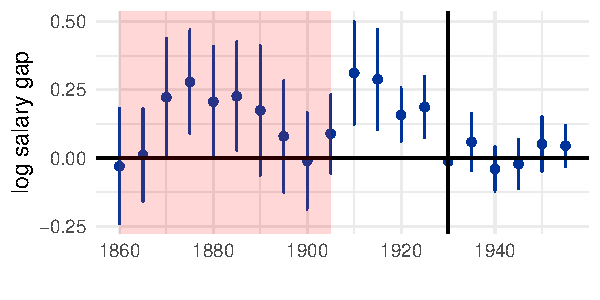
\includegraphics[width=\maxwidth]{figure/plot3-1} 

}

\caption[Salary gap and the removal of patronage on basis of the regression of column (2) in Table 4]{Salary gap and the removal of patronage on basis of the regression of column (2) in Table 4. Red shaded area: Years not shown in the original plot in the paper.}\label{fig:plot3}
\end{figure}



\subsection{Performance and connectedness}
\hspace*{5mm} In Table~\ref{tab:rev}, we see the replication of panel A of Table 5 in the paper (the effect of connectedness on colony revenues), and in Table~\ref{tab:exp} the replication of panel B (the effect of connectedness on colony expenditure). Both revenues and expenditures serve as measures of governors' job performance. For Table~\ref{tab:rev}, the sum of the coefficients of the connected dummy and the interaction between being connected and being after 1930 (column 2) is 0.006 with a standard error of 0.027. The respective sum and standard error for Table~\ref{tab:exp} are 0.011 and 0.025. We therefore see that after the Warren-Fisher reform, both the differentials in revenue and expenditures vanish. I reproduce column (2) in both tables will the complete dataset in column (5), respectively and find no qualitative difference. The combined effects $Connected + Reform*Connected$ are -0.012 (0.028) for revenues and -0.003 (0.028) for expenditures. Therefore, also with all data included, the performance gap closes with the reform.

% Table created by stargazer v.5.2.3 by Marek Hlavac, Social Policy Institute. E-mail: marek.hlavac at gmail.com
% Date and time: Wed, Sep 27, 2023 - 2:58:27 PM
\begin{table}[!htbp] \centering 
  \caption{The effects of connectedness on colony revenue and its components} 
  \label{tab:rev} 
\scriptsize 
\begin{tabular}{@{\extracolsep{5pt}}lccccc} 
\\[-1.8ex]\hline 
\hline \\[-1.8ex] 
 & \multicolumn{5}{c}{log revenue} \\ 
\cline{2-6} 
 & \multicolumn{2}{c}{Total} & Trade & Internal & All \\ 
\\[-1.8ex] & (1) & (2) & (3) & (4) & (5)\\ 
\hline \\[-1.8ex] 
 No. colonies served & 0.078 & 0.077 & $-$0.025 & 0.235$^{***}$ & 0.067 \\ 
  & (0.060) & (0.060) & (0.048) & (0.091) & (0.057) \\ 
  & & & & & \\ 
 Connected & $-$0.040$^{**}$ & $-$0.055$^{***}$ & $-$0.053$^{**}$ & $-$0.043 & $-$0.051$^{**}$ \\ 
  & (0.017) & (0.021) & (0.026) & (0.032) & (0.022) \\ 
  & & & & & \\ 
 Reform x Connected &  & 0.061$^{*}$ &  &  & 0.039 \\ 
  &  & (0.033) &  &  & (0.035) \\ 
  & & & & & \\ 
\hline \\[-1.8ex] 
Mean of dep. var & 12.309 & 12.309 & 11.499 & 11.625 &  \\ 
Year FE & Yes & Yes & Yes & Yes & Yes \\ 
Governor-Colony FE & Yes & Yes & Yes & Yes & Yes \\ 
Spell lengths FE & Yes & Yes & Yes & Yes & Yes \\ 
Observations & 3,510 & 3,510 & 2,708 & 2,698 & 3,885 \\ 
\hline 
\hline \\[-1.8ex] 
\textit{Note:}  & \multicolumn{5}{r}{$^{*}$p$<$0.1; $^{**}$p$<$0.05; $^{***}$p$<$0.01} \\ 
\end{tabular} 
\end{table} 

% Table created by stargazer v.5.2.3 by Marek Hlavac, Social Policy Institute. E-mail: marek.hlavac at gmail.com
% Date and time: Wed, Sep 27, 2023 - 2:58:27 PM
\begin{table}[!htbp] \centering 
  \caption{The effects of connectedness on colony expenditures and their components} 
  \label{tab:exp} 
\scriptsize 
\begin{tabular}{@{\extracolsep{5pt}}lccccc} 
\\[-1.8ex]\hline 
\hline \\[-1.8ex] 
 & \multicolumn{5}{c}{log expenditure} \\ 
\cline{2-6} 
 & \multicolumn{2}{c}{Total} & Tax & Works & All \\ 
\\[-1.8ex] & (1) & (2) & (3) & (4) & (5)\\ 
\hline \\[-1.8ex] 
 No. colonies served & 0.093$^{*}$ & 0.091 & 0.049 & 0.055 & 0.092$^{*}$ \\ 
  & (0.056) & (0.056) & (0.270) & (0.106) & (0.054) \\ 
  & & & & & \\ 
 Connected & $-$0.029 & $-$0.042$^{*}$ & $-$0.089$^{*}$ & $-$0.107$^{*}$ & $-$0.041$^{*}$ \\ 
  & (0.019) & (0.023) & (0.054) & (0.062) & (0.024) \\ 
  & & & & & \\ 
 Reform x Connected &  & 0.053 &  &  & 0.038 \\ 
  &  & (0.034) &  &  & (0.036) \\ 
  & & & & & \\ 
\hline \\[-1.8ex] 
Mean of dep. var & 12.333 & 12.333 & 9.016 & 10.317 & 12.236 \\ 
Year FE & Yes & Yes & Yes & Yes & Yes \\ 
Governor-Colony FE & Yes & Yes & Yes & Yes & Yes \\ 
Spell lengths FE & Yes & Yes & Yes & Yes & Yes \\ 
Observations & 3,510 & 3,510 & 1,754 & 2,606 & 3,826 \\ 
\hline 
\hline \\[-1.8ex] 
\textit{Note:}  & \multicolumn{5}{r}{$^{*}$p$<$0.1; $^{**}$p$<$0.05; $^{***}$p$<$0.01} \\ 
\end{tabular} 
\end{table} 

\hspace*{5mm} I refrain from including a reproduction of Figure 5 into this excercise, because -- unlike Figure~\ref{fig:plot3} -- it represents estimates from a naive staggered DiD estimation as it was standard before \cite{sun2021} and related papers. That is, estimates shown in this figure will only be unbiased if all of the following assumptions hold simultaneously:
\begin{enumerate}
  \item parallel trends
  \item no anticipation
  \item homogeneous treatment effects
\end{enumerate}
\hspace*{5mm} At least the third assumption is very implausible to hold as, while connectedness is a dummy variable in the present dataset, in reality might it vary in degree and nature. Not only might one governor have a stronger bond of friendship with the incumbent secretary of state than another governor -- even if they all went to the same university. In few cases, connectedness might also even yield the opposite effect: Secretaries might be on bad terms with some governors, denying them e.g. a transfer to a higher paying colony that they would have gotten otherwise. \cite{callaway2021} have come forward with an estimator that allows for heterogeneous treatment effects which is even implemented in an \texttt{R} package but not estimable with this particular dataset because the data on different treatment groups (mandates of governors) do not overlap. That is, the long time span from 1854 until 1966 in combination with the rather short mandate timespans per governor does not allow for the interpretation as an unbalanced panel, which is crucial for this estimator. Fortunately, Figure 5 is not a main result of \cite{guoxu2018} but rather a dynamic illustration of what is shown in Table~\ref{tab:rev} and \ref{tab:exp} anyway: Governors reduce expenditure and revenue as they get connected which a secretary of state.    

\subsection{Ordinances and exemptions}
\hspace*{5mm} Tables~\ref{tab:ord} and \ref{tab:combo_ord} show the replication of Table 6 in the paper, which studies tax exemptions and ordinances in response to connectedness. As governors had far-reaching discretion in tax matters of the colony and tax avoidance denoted a means of personal enrichment (of themselves or other members of the settler elite), their tax policy denotes a particularly fitting area to study when it comes to connectedness under patronage. We see indeed significantly more ordinances for connected governors in total (column 1), which appears to be significantly driven by more exemptions (4) and ordinances on tariff (3), both policies to disproportionally affect the settler elite. This gap between connected and unconnected governors then disappears after 1930, and no gap can be found for other taxes (2), social programs (5) and public works (6).

% Table created by stargazer v.5.2.3 by Marek Hlavac, Social Policy Institute. E-mail: marek.hlavac at gmail.com
% Date and time: Wed, Sep 27, 2023 - 2:58:27 PM
\begin{table}[!htbp] \centering 
  \caption{Tax ordinances, exemptions and connectedness to the Secretary of State} 
  \label{tab:ord} 
\scriptsize 
\begin{tabular}{@{\extracolsep{5pt}}lcccccc} 
\\[-1.8ex]\hline 
\hline \\[-1.8ex] 
 & Total & Direct tax & Customs & Exemptions & Social & Works \\ 
\\[-1.8ex] & (1) & (2) & (3) & (4) & (5) & (6)\\ 
\hline \\[-1.8ex] 
 No. colonies served & $-$0.009 & $-$0.006 & 0.001 & 0.510 & $-$0.005 & $-$0.009 \\ 
  & (0.016) & (0.013) & (0.010) & (0.320) & (0.013) & (0.009) \\ 
  & & & & & & \\ 
 Connected & 0.085$^{**}$ & 0.048 & 0.068$^{**}$ & 0.202$^{***}$ & 0.004 & $-$0.011 \\ 
  & (0.038) & (0.031) & (0.031) & (0.064) & (0.028) & (0.020) \\ 
  & & & & & & \\ 
 Reform x Connected & $-$0.083$^{**}$ & $-$0.051 & $-$0.066$^{**}$ & $-$0.369$^{***}$ & $-$0.003 & 0.013 \\ 
  & (0.038) & (0.032) & (0.031) & (0.139) & (0.029) & (0.019) \\ 
  & & & & & & \\ 
\hline \\[-1.8ex] 
Mean of dep. var & 0.021 & 0.01 & 0.014 & 0.226 & 0.012 & 0.007 \\ 
Year FE & Yes & Yes & Yes & Yes & Yes & Yes \\ 
Governor-Colony FE & Yes & Yes & Yes & Yes & Yes & Yes \\ 
Spell lengths FE & Yes & Yes & Yes & Yes & Yes & Yes \\ 
Observations & 581 & 581 & 581 & 421 & 581 & 581 \\ 
\hline 
\hline \\[-1.8ex] 
\textit{Note:}  & \multicolumn{6}{r}{$^{*}$p$<$0.1; $^{**}$p$<$0.05; $^{***}$p$<$0.01} \\ 
\end{tabular} 
\end{table} 
\begin{table}[!h]

\caption{\label{tab:combo_ord}Being connected after 1930, ordinances and exemptions}
\centering
\fontsize{7}{9}\selectfont
\begin{tabular}[t]{lrrrrrr}
\toprule
  & (1) & (2) & (3) & (4) & (5) & (6)\\
\midrule
Estimate & 0.002 & -0.003 & 0.002 & -0.167 & 0.001 & 0.002\\
SE & 0.006 & 0.005 & 0.004 & 0.128 & 0.005 & 0.003\\
\bottomrule
\end{tabular}
\end{table}



\subsection{Additional performance measures}
\hspace*{5mm} Lastly, Tables~\ref{tab:alt} and \ref{tab:combo_alt} reproduce Table 7 from the paper on alternative performance measures and connectedness, namely mentions of social unrest in the colony in British newspapers (1), mentions of certain governors in text-mined parliament speeches (2) and sentiments in these speeches (3), and receipt of public awards (4). All included measures except (2) imply that connected governors performed worse during the time of patronage. I augment these tables again by the inclusion of all observations for social unrest (5) and sentiment (6). Social unrest now turns insignificant (i.e. no difference between connected and unconnected even before abolishment), while sentiment stays significant at a 10\% level.

% Table created by stargazer v.5.2.3 by Marek Hlavac, Social Policy Institute. E-mail: marek.hlavac at gmail.com
% Date and time: Wed, Sep 27, 2023 - 2:58:27 PM
\begin{table}[!htbp] \centering 
  \caption{Alternative performance measures and connectedness to the Secretary of State} 
  \label{tab:alt} 
\scriptsize 
\begin{tabular}{@{\extracolsep{5pt}}lcccccc} 
\\[-1.8ex]\hline 
\hline \\[-1.8ex] 
 & Unrest & Mentions & Sentiment & Awards & Unrest (All) & Sentiment (All) \\ 
\\[-1.8ex] & (1) & (2) & (3) & (4) & (5) & (6)\\ 
\hline \\[-1.8ex] 
 No. colonies served & $-$0.005 & 0.111$^{*}$ & 0.026 & 0.082 & 0.110$^{**}$ & $-$0.003 \\ 
  & (0.037) & (0.065) & (0.052) & (0.080) & (0.055) & (0.034) \\ 
  & & & & & & \\ 
 Connected & 0.038$^{*}$ & 0.029 & $-$0.045$^{*}$ & $-$0.031$^{**}$ & 0.032 & $-$0.040$^{*}$ \\ 
  & (0.022) & (0.028) & (0.024) & (0.015) & (0.021) & (0.024) \\ 
  & & & & & & \\ 
 Reform x Connected & $-$0.037$^{*}$ & $-$0.040 & 0.039 & $-$0.007 & $-$0.030 & 0.043$^{*}$ \\ 
  & (0.022) & (0.031) & (0.029) & (0.028) & (0.020) & (0.025) \\ 
  & & & & & & \\ 
\hline \\[-1.8ex] 
Mean of dep. var & 0.05 & 0.724 & 0.1 & 0.022 & 0.045 & 0.094 \\ 
Year FE & Yes & Yes & Yes & Yes & Yes & Yes \\ 
Governor-Colony FE & Yes & Yes & Yes & Yes & Yes & Yes \\ 
Spell lengths FE & Yes & Yes & Yes & Yes & Yes & Yes \\ 
Observations & 3,510 & 3,510 & 2,542 & 3,510 & 4,644 & 3,308 \\ 
\hline 
\hline \\[-1.8ex] 
\textit{Note:}  & \multicolumn{6}{r}{$^{*}$p$<$0.1; $^{**}$p$<$0.05; $^{***}$p$<$0.01} \\ 
\end{tabular} 
\end{table} 
\begin{table}[!h]

\caption{\label{tab:combo_alt}Being connected after 1930, alternative measures}
\centering
\fontsize{7}{9}\selectfont
\begin{tabular}[t]{lrrrrrr}
\toprule
  & (1) & (2) & (3) & (4) & (5) & (6)\\
\midrule
Estimate & 0.001 & -0.011 & -0.007 & -0.037 & 0.002 & 0.003\\
SE & 0.002 & 0.015 & 0.017 & 0.024 & 0.001 & 0.009\\
\bottomrule
\end{tabular}
\end{table}



\section{Conclusion}
\cite{guoxu2018} is a very strong paper that provides very compelling and easily tractable evidence for the argument of patronage being a suboptimal way of organizing public policy. None of my additionally conducted robustness checks was able to weaken the fundamental evidence in this paper. However, it has to be kept in mind that much of my analysis is dependent on the provided dataset, which was composed by the author himself. That is, although the evidence from this paper and excercise is indeed very compelling, I have no insight into the selection of variables made beforehand. 

\section{References}
\printbibliography[heading=none]

\end{document}
